
\section{Atwood's Machine\footnote{
1990-93 Dept. of Physics and Astronomy, Dickinson College. Supported by FIPSE
(U.S. Dept. of Ed.) and NSF. Portions of this material may have been modified
locally and may not have been classroom tested at Dickinson College.
}}

Name \rule{2.0in}{0.1pt}\hfill{}Section \rule{1.0in}{0.1pt}\hfill{}Date \rule{1.0in}{0.1pt}

\textbf{Objective }

To apply tension concepts and Newton's laws of motion to the analysis of Atwood's
machine.

\textbf{Overview }

Sometime before 1780, a physicist at Cambridge University named George Atwood
devised a marvelous machine for measuring the acceleration of a falling mass
without the aid of high speed timers, motion detectors, or video cameras. It
consists of two masses connected to each other by means of a light string passing
over a relatively frictionless light pulley, as shown in the diagram below.

\vspace{0.3cm}
{\par\centering 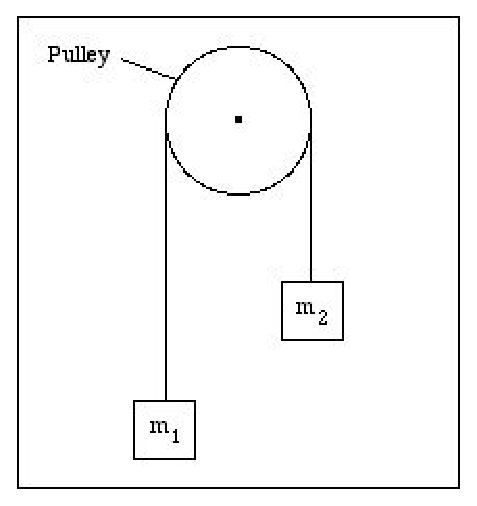
\includegraphics{atwood_fig1.eps} \par}
\vspace{0.3cm}

Atwood's machine is not only historically important but it allows us to practice
applying Newton's laws and the kinematic equations to the analysis of motion.

\textbf{Apparatus} 

\begin{itemize}
\item Smart pulley with photogate 
\item String with 2 hooks 
\item Small washers (15)
\item \textit{Science Workshop 750 Interface}
\item \textit{DataStudio} software (Atwood's Machine application)
\end{itemize}
\textbf{Activity 1: Predictions and Qualitative Observations} 

(a) Assume that the two masses are equal. If you pull down gently on one of
them, what motion do you predict will result? Explain your reasoning.
\vspace{20mm}

(b) Set up Atwood's Machine with combinations of equal masses (same number of
washers on each hook), pull on one of them gently, and describe what you observe.
How does your observation compare with your prediction?
\vspace{20mm}

(c) Suppose that \( m_{1} \) is greater than \( m_{2} \). What do you expect
to observe and why?
\vspace{20mm}

(d) Set up Atwood's Machine with combinations of unequal masses, and describe
what you observe. How do your observations compare with your prediction?
\vspace{20mm}

\textbf{Activity 2: Quantitative Observations }

(a) Perform the following procedure to measure the acceleration of Atwood's
machine for different combinations of masses. 

1. Determine and record the mass of the two wire hooks using a laboratory balance.
\vspace{10mm}

2. Determine and record the mass of fifteen (15) washers. Calculate and record
the average mass of one washer.
\vspace{10mm}

3. Construct a data table below with the column headings: Trial \#, \( m_{1} \),
\( m_{2} \), \( m_{1}  - m_{2} \), Experimental Acceleration, Theoretical
Acceleration, and \% Difference. Leave enough room to record data for seven
trials.
\vspace{50mm}

4. Launch the Atwood's Machine application.

5. Place eight washers on one wire hook and seven on the other. Record the appropriate
values in your data table including the masses of the wire hooks. Let \( m_{1} \)
be the heavier mass. 

6. Move \( m_{1} \) upward until \( m_{2} \) almost touches the floor. Make
sure the string is over the pulley and that the two masses are motionless. 

7. Start recording data and release \( m_{1} \), which will fall downward,
pulling \( m_{2} \) up. The computer will display a graph of velocity versus
time. Fit the data with a straight line. The slope of the line and mean-squared
error (MSE) of the fit will also be displayed. Examine the graph. If you feel
the line provides a good fit to the data, record the slope in your data table.
This is the acceleration in units of m/s\( ^{2} \). If the fit is not good,
repeat the run. 

8. Move one washer from \( m_{2} \) to \( m_{1} \), record the appropriate
masses in your data table, and repeat steps 6 and 7. Note that the total mass
of the system remains constant. 

9. Repeat step 8 until \( m_{2} \) consists of only one washer (and one wire
hook). You will have a total of seven trials.

(b) Construct a graph of experimental acceleration (vertical axis) versus \( m_{1}  - m_{2} \) (horizontal axis). Find the best fit to the data to determine the mathematical relationship between the mass difference and the acceleration. Print the graph showing the fit and put a copy in your notebook. Write the equation (with appropriate units) that describes the data in the space below.
\vspace{20mm}

\textbf{Activity 3: Derivation of Atwood's Equation }

(a) If the tension on the string is denoted by $T$, draw a diagram describing
the forces on \( m_{1} \). Draw another diagram showing the forces on \( m_{2} \).
Hint: Include the gravitational forces acting in the negative y-direction on
masses 1 and 2 and the tension forces acting upwards. Assume that \( m_{1} \)
is greater than \( m_{2} \).
\vspace{20mm}

(b) Write down an equation for the net force on \( m_{1} \) in terms of $T$, $g$, and \( m_{1} \). Use Newton's second law to relate this net force to the acceleration, \( a_{1} \), of \( m_{1} \).
\vspace{20mm}

(c) Next, write down an equation for the net force on \( m_{2} \) in terms
of $T$, $g$, and \( m_{2} \). Use Newton's second law to relate this net force
to the acceleration \( a_{2} \) of \( m_{2} \). 
\vspace{20mm}

(d) Why can we say the acceleration of \( m_{1} \) is \( a_{1} = -a\) if
the acceleration of \( m_{2} \) is \( a_{2} = a\)?
\vspace{20mm}

(e) Eliminate $T$ from the two equations to show that the net acceleration for
the Atwood's machine is given by the equation \( a=\frac{m_{1}-m_{2}}{m_{1}+m_{2}}g \). 
\vspace{40mm}

(f) You have just derived the famous Atwood's equation. Use this expression
to calculate the theoretical acceleration for each trial and record the values
in the table in Activity 2.

(g) Compare the experimental acceleration with the theoretical acceleration
by determining the \% difference between the two for each trial. Is there good
agreement between the two values? Do the results verify Newton's Second Law
of motion? Is there a systematic difference? If so, what might this be due to?
\vspace{20mm}

(h) Rearrange the expression you derived for the acceleration so that it is
the equation of the graph you constructed in Activity 2. Note that the slope
of the graph contains g. Calculate g from the slope determined from your fit
and find the \% difference between this value and the accepted value. How well
do the two values agree? Can you account for any difference?

